\chapter{Código fonte de um Universo Conceitual como nuvem de palavras sobre o improviso de códigos}\label{app:A}

O tema da improvisação de códigos, como um universo de conceitos, surgiu de uma experiência com um código em linguagem \emph{python}\disponivelem{https://www.python.org/}, útil para gerar um mapa de termos, como ilustrado na figura \autoref{fig:nuvemlivecoding}

\begin{figure}[!h]
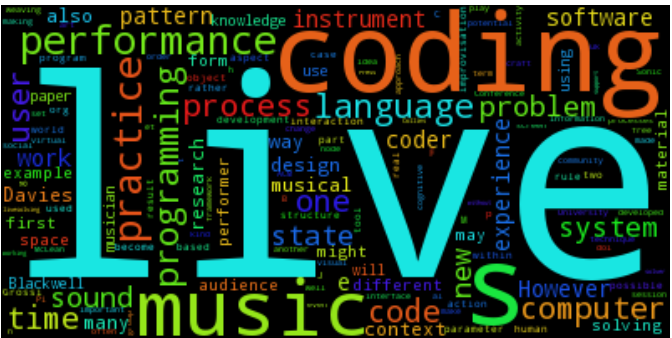
\includegraphics[scale=0.8]{imagens/nuvem.png}
\caption{Nuvem de palavras do \citeonline{ICLC2015},  1$^o$ Congresso Internacional de Live Coding. \textbf{Fonte}: autor.}
\label{fig:nuvemlivecoding}
\end{figure}

A imagem acima foi gerada com um código nomeado como \emph{cloupdf.py}, e considera seguinte situação, subdividida em três passos: 

1) Converter um arquivo de texto, ou um conjunto de textos cientítificos, em formato \emph{.pdf} para formato \emph{.txt}; 

2) Feita a conversão, plotar uma imagem com as palavras mais relevantes, do ponto de vista quantitativo; 

3) Desta plotagem, organizar as palavras qualitativamente, de acordo com suas funções gramaticais no texto, em classes quantitativas (ver \autoref{tab:gen1}, p.~\pageref{tab:gen1}; \autoref{tab:gen2}, p.~\pageref{tab:gen2}; \autoref{tab:gen3}, p.~\pageref{tab:gen3}; \autoref{tab:gen4}, p.~\pageref{tab:gen4}; \autoref{tab:gen5}, p.~\pageref{tab:gen5}).

\begin{example}{Código-fonte do \emph{cloud.py}}
\begin{minted}[fontsize=\scriptsize]{python}
#!/usr/bin/python

# Algumas bibliotecas principais
from wordcloud import WordCloud     # Nuvem de palavras
import nltk                         # Processamento de linguagem natural
import matplotlib.pyplot as plt     # Desenha foto
from subprocess import Popen, PIPE  # Acessa um o conversor de pdf
from optparse import OptionParser   # Cria um programa

# Bibliotecas basicas
from os import path
import math

# PROGRAMA PRINCIPAL
def linha_de_comando(nome, versao, descricao): 
    parser = OptionParser(usage='usage: %prog [OPTIONS, [ARGS]]', 
                          version='%s %s' % (nome, versao), 
                          description=descricao)
    # Cria opcoes
    parser.add_option("-e","--entrada",
                      action=None,
                      help="arquivo pdf de entrada",
                      dest="input",default=False)
    parser.add_option("-q","--qualidades",
                      action=None,
                      help="classificacao por qualidades (0..n-1)",
                      dest="qualidades",
                      default=False)
    parser.add_option("-f","--foto",
                      action="store_true", 
                      help="arquivo de saida da foto",
                      dest="fotinha",
                      default=False),
    parser.add_option("-p","--paginas",
                      action=None,
                      help="paginas processadas",
                      dest="paginas",
                      default=False)
    parser.add_option("-c","--codec",
                      action=None,
                      help="tipo de codificacao do texto",
                      dest="codec",
                      default=False)
    parser.add_option("-t","--table",
                      action=None,
                      help="converte a nuvem para uma tabela: \n\t-tex (suportado)\n\t-mardown (planejado)",
                      dest="table",
                      default=False)

    # Life cycle
    (options, args) = parser.parse_args()
    pages = []
    if options.paginas:
        split =  options.paginas.split("..") 
        a = [ str(s) for s in range(int(split[0]), int(split[1])) ]
        pages = ",".join(a)
    else:
        pages = [1,2]
    text = convert_pdf_to_txt(options.input,pages,options.codec)
    
    # Nuvem
    print "\n\nA gerar nuvem ..."
    nuvem = WordCloud().generate(text)
    print "=> Feito"
    if options.fotinha:
        gera_figura(nuvem)
    
    #if options.table:
    # Taggins
    print "\n\nA classificar e organizar palavras em uma tabela"
    tagging = nltk.pos_tag(nltk.word_tokenize(text))
    qualidades = gera_grupos_qualitativos(nuvem, tagging, int(options.qualidades) or 10)
    nome = options.input.split(".tex")[0]
    f = open("%s.tex" % options.table, "w+")

    #    if options.table is "tex":
    tabela_tex = table(qualidades, options.qualidades, options.table, "tab:gen").decode(options.codec)
    f.write(tabela_tex)
    f.close()
    print "=> Feito: %s.tex" % options.table
    
#http://davidmburke.com/2014/02/04/python-convert-documents-doc-docx-odt-pdf-to-plain-text-without-libreoffice/
#http://stackoverflow.com/questions/5725278/python-help-using-pdfminer-as-a-library
def convert_pdf_to_txt(p, pages, codec):
    name = p.split(".pdf")[0].split("/")[-1]
    _path = path.abspath("%s.txt") % name
    print "A converter %s para %s  ... \n\n" % (p,_path)
    command = "=> pdf2txt.py -o %s -p %s -c %s %s" % (_path, pages, codec, p)
    print command
    #https://stackoverflow.com/questions/24340877/why-does-this-bash-call-from-python-not-work
    result = Popen(command, stdout=PIPE, shell=isinstance(command, str))
    #print result.communicate()
    print "=> ... checking ascii characters"
    f = open(_path)
    s = ""
    for i, line in enumerate(f.readlines()):
        l = line.decode(codec)
        s += l

    print "=> Feito"
    return s
    
# gera figura a partir da nuvem
def gera_figura(nuvem):
    print "A gerar uma nuvem de palavras..."
    plt.figure()
    plt.imshow(nuvem)
    plt.axis("off")
    print "=> Pronto"
    plt.show()
    
###
# CC: conjunction, coordinating
# CD: numeral, cardinal
# DT: determiner
# EX: existential there
# FW: foreign word
# IN: preposition or conjunction, subordinating
# JJ: adjective or numeral, ordinal
# JJR: adjective, comparative
# JJS: adjective, superlative
# LS: list item marker
# MD: modal auxiliary
# NN: noun, common, singular or mass
# NNP: noun, proper, singular
# NNPS: noun, proper, plural
# NNS: noun, common, plural
# PDT: pre-determiner
# POS: genitive marker
# PRP: pronoun, personal
# PRP$: pronoun, possessive
# RB: adverb
# RBR: adverb, comparative
# RBS: adverb, superlative
# RP: particle
# SYM: symbol
# UH: interjection
# VB: verb, base form
# VBD: verb, past tense
# VBG: verb, present participle or gerund
# VBN: verb, past participle
# VBP: verb, present tense, not 3rd person singular
# VBZ: verb, present tense, 3rd person singular
# WDT: WH-determiner
# WP: WH-pronoun
# WP$: WH-pronoun, possessive
# WRB: Wh-adverb
###
def criaGrupos(nuvem, tagging, n, groups={}):
    # primeiro crie uma tabela das funcoes:
    for tag in tagging:
        if not str(tag[1]) in groups:
            groups.__setitem__(tag[1], {})
        
        for t in nuvem.words_:
            freq = t[1]
            index = int(math.floor(freq*n))
            if not str(index) in groups.__getitem__(tag[1]):
                groups.__getitem__(tag[1]).__setitem__(str(index), [])

            word = t[0].title()
            t = tag[0].title()
            if word == t:
                if not word in groups.__getitem__(tag[1]).__getitem__(str(index)):
                    groups.__getitem__(tag[1]).__getitem__(str(index)).append(word)

        for i in range(n):
            if not str(i) in groups.__getitem__(tag[1]):
                groups.__getitem__(tag[1]).__setitem__(str(i), [])
                
    return groups

def gera_grupos_qualitativos(nuvem, tagging, n):
    return criaGrupos(nuvem, tagging, n)

def table(groups, size, caption, label):
    print "=> creating table for %s" % caption
    print groups
    string =  """\\begin{table}
\\centering
\\caption{%s}
\\label{%s}
\\small
\\begin{tabular}{""" % (caption, label)
    string = string + "%s" % "".join([" | p{1cm}" for i in range(int(size)+2)])
    string = string + """ |}
\\hline
\\hline
"""
    # Cabecalho geral
    string = string+ "\\tiny \\textbf{Qualidade/Funcao}\n"
    for i in range(int(size)):
        if i is not int(size)-1:
            string = string + " & \\textbf{%s}\n" % i
        else:
            string = string + " & \\textbf{%s} \\\\ \n" % i
    string = string + "\\hline\n\\hline\n"

    # conteudo again:
    for k, v in groups.iteritems():
        string = string + "\\tiny \\textbf{%s}\n" % k 
        a = range(int(size)+1)
        for i in a:
            string = string + " & \\tiny"
            if len(v[str(i)]) is 0:
                string = string + " -- "
            else:
                string = string + " %s " % ", ".join(v[str(i)])
    
            if i is len(a) :
                string = string + " \\\\ \n"
        string = string + "\\hline\n"
            
    string = string +  """
\\hline
\\end{tabular}
\\end{table}
"""
    print string
    return string
    
linha_de_comando("claudio", "0.0.1", "Script python para gerar nuvem de arquivos pdf")


\end{minted}
\end{example} 

\section{Utilização}

Em um terminal Linux (3.16.0-49-generic, Ubuntu 14.04.1, i686), executamos o código como um comando  com opções de: 1) arquivo de entrada (\verb|--entrada| ou \verb|-e|), número de páginas rastreadas (\verb|--paginas| ou \verb|-p|), classes (\verb|--qualidades| ou \verb|-q|), codificação do pdf (\verb|--codec| ou \verb|-c|), criação de uma nuvem de palavras (\verb|--foto| ou \verb|-f|) e organização de uma tabela (\verb|--table| ou \verb|-t|). 

Este código utilizou três bibliotecas auxiliares \emph{pdf2text.py}\disponivelem{https://pypi.python.org/pypi/pdf2text}, \emph{Wordcloud}\disponivelem{https://github.com/amueller/word_cloud} e \emph{NLTK}\disponivelem{http://nltk.org/}. 

A primeira biblioteca permite extrair do pdf caracteres válidos para análise. A segunda biblioteca realiza o levantamento de dados. E a terceira biblioteca auxilia na organização das funções gramaticais. Essas operações serão exemplificadas na próxima seção.

\section{Experiências}

Durante uma primeira experiência, abrimos um arquivo pdf, mais especificamente os anais de um congresso internacional \cite{ICLC2015}, e organizamos algumas páginas pertinentes, neste caso, todas a páginas com o corpo de texto (p. 4 -- 230),  supostamente codificado em um padrão ISO8895-1 \ver{fig:nuvemlivecoding}.

\begin{example}{Código-fonte do \emph{cloud.py}}
\begin{minted}[fontsize=\scriptsize]{bash}
./cloud.py -e ./iclc2015-proceedings.pdf -p 4..231 -f
\end{minted}
\end{example} 

Uma segunda experiência permitiu organizar a mesma nuvem de palavras em um uma tabela de funções gramaticais. As duas experiências dispararam a intenção de realizar uma pesquisa onde fosse possível verificar os mesmos conceitos em uma bibliografia geral, como feita nos \autoref{cap:introducao} e \autoref{sec:protohistoria}.

\begin{example}{Código-fonte do \emph{cloud.py}}
\begin{minted}[fontsize=\scriptsize]{bash}
./cloud.py -e ./iclc2015-proceedings.pdf -q 10 -p 4..231 -c iso8859-1 -t tex
\end{minted}
\end{example} 

A execução do comando acima gera a seguinte saída de texto:

\begin{example}{Saída de texto do \emph{cloud.py}}
\begin{minted}[fontsize=\scriptsize]{bash}
A converter ./iclc2015-proceedings.pdf para ./iclc2015-proceedings.txt  ... 

=> pdf2txt.py -o /home/guilherme/bitbucket/mestrado/iclc2015-proceedings.txt 
-p 4,5,6,7,8,9,10,11,12,13,14,15,16,17,18,19,20,21,22,23,24,25,26,27,28,29,30,31,
32,33,34,35,36,37,38,39,40,41,42,43,44,45,46,47,48,49,50,51,52,53,54,55,56,57,58,
59,60,61,62,63,64,65,66,67,68,69,70,71,72,73,74,75,76,77,78,79,80,81,82,83,84,85,
86,87,88,89,90,91,92,93,94,95,96,97,98,99,100,101,102,103,104,105,106,107,108,109,
110,111,112,113,114,115,116,117,118,119,120,121,122,123,124,125,126,127,128,129,130,
131,132,133,134,135,136,137,138,139,140,141,142,143,144,145,146,147,148,149,150,151,
152,153,154,155,156,157,158,159,160,161,162,163,164,165,166,167,168,169,170,171,172,
173,174,175,176,177,178,179,180,181,182,183,184,185,186,187,188,189,190,191,192,193,
194,195,196,197,198,199,200,201,202,203,204,205,206,207,208,209,210,211,212,213,214,
215,216,217,218,219,220,221,222,223,224,225,226,227,228,229,230 
-c iso8859-1 /home/guilherme/Dropbox/Mestrado/livecoding/iclc2015-proceedings.pdf
=> ... checking ascii characters
=> Feito

A gerar nuvem ...
=> Feito

A classificar e organizar palavras em uma tabela
=> Feito
\end{minted}
\end{example}

\newpage

\begin{table}
\centering
\caption{VB -- Verbo, forma básica. VBZ -- presente na terceira pessoa do singular.}
\label{tab:gen1}
\small
\begin{tabular}{ | p{2.6cm} | p{2.1cm} | p{2.1cm} | p{1.5cm} | p{0.5cm} | p{0.5cm} | p{0.25cm} | p{0.25cm} | p{0.25cm} | p{0.25cm} | p{0.25cm} | p{0.75cm} |}
\hline
\hline
\tiny \textbf{Qualidade/Função}
 & \textbf{0}
 & \textbf{1}
 & \textbf{2}
 & \textbf{3}
 & \textbf{4}
 & \textbf{5}
 & \textbf{6}
 & \textbf{7}
 & \textbf{8}
 & \textbf{9}
 & \textbf{10} \\ 
\hline
\hline
\tiny \textbf{VB} & \tiny See, Take, Allow, Make, Explore, Provide, Change, Support, Result, Become, Play, Create, Set, Laptop, Show, Project, Different, Type, Output, Object, Present, Point, Parameter, Structure, Memory, Need, Feature, Cognitive, Open, Interface, End, Text, C, Working, Control, Musician, Form, Line, Technique, Ensemble, Networked  & \tiny Use, Design, Machine, Work, State, Problem, Experience, Audio  & \tiny Sound, User, Time, Practice  & \tiny E  & \tiny Code  & \tiny --  & \tiny --  & \tiny --  & \tiny --  & \tiny --  & \tiny Live \\ 
\hline
\tiny \textbf{VBZ}
 & \tiny Collins  & \tiny --  & \tiny --  & \tiny --  & \tiny --  & \tiny --  & \tiny --  & \tiny --  & \tiny --  & \tiny --  & \tiny -- \\
 \hline
 \hline
\end{tabular}
\end{table}

É possível notar possíveis erros de organização das palavras com a utilização da biblioteca NLTK. Isso é notável com a inclusão erros ortográficos \ver{tab:gen1} e var{tab:gen2}, ou inclusão de substantivos como um verbo \ver{tab:gen1}, ou adjetivos como verbos \ver{tab:gen3}.

O primeiro tipo de erro pode ocorrer como um erro de método de codificação (ISO 8895-1). 
 
 O segundo tipo de erro pode ocorrer pela definição de regras gramaticais, ao qual usamos um padrão,  a função \verb|nltk.word_tokenize| (ver  \autoref{ex:cloud}, p.~\pageref{ex:cloud}), dentre diversos possíveis\disponivelem{http://stackoverflow.com/questions/24975573/how-to-parse-custom-tags-using-nltk-regexp-parser}. 

\begin{table}
\centering
\caption{VBG -- \emph{present participle}. VBD -- \emph{past tense}. VBN -- \emph{past participle}}
\label{tab:gen2}
\small
\begin{tabular}{ | p{2.6cm} | p{2.6cm} | p{1.75cm} | p{1.75cm} | p{0.25cm} | p{0.25cm} | p{0.25cm} | p{1cm} | p{0.25cm} | p{0.25cm} | p{0.25cm} | p{0.25cm} |}
\hline
\hline
\tiny \textbf{Qualidade/Função}
 & \textbf{0}
 & \textbf{1}
 & \textbf{2}
 & \textbf{3}
 & \textbf{4}
 & \textbf{5}
 & \textbf{6}
 & \textbf{7}
 & \textbf{8}
 & \textbf{9}
 & \textbf{10} \\ 
\hline
\hline
\tiny \textbf{VBG}
 & \tiny Working, Making, Livecoding, Solving  & \tiny Using, Writing  & \tiny Programming  & \tiny --  & \tiny --  & \tiny --  & \tiny Coding  & \tiny --  & \tiny --  & \tiny --  & \tiny -- \\
\hline
\tiny \textbf{VBD}
 & \tiny Set, Developed, Made, Concept, Networked, Shared, Output, Become, Dierent  & \tiny Used, Instrument, Based  & \tiny Sound  & \tiny --  & \tiny --  & \tiny --  & \tiny --  & \tiny --  & \tiny --  & \tiny --  & \tiny -- \\
\hline
\tiny \textbf{VBN}
 & \tiny Developed, Made, Become, Shared, Networked, Method, Set, Need, Output  & \tiny Used, Based  & \tiny --  & \tiny --  & \tiny --  & \tiny --  & \tiny --  & \tiny --  & \tiny --  & \tiny --  & \tiny -- \\
 \hline
  \hline
\end{tabular}
\end{table}

Dado estes erros gramaticais, sugerimos observar algumas palavras, de acordo com uma polimorfia (se a palavra aparece ou não em várias das classes), ou seu grau na escala. Neste sentido \emph{Live} aparece tanto como verbo \ver{tab:gen1} e \ver{tab:gen2}, adjetivo \ver{tab:gen3} e substantivo \ver{tab:gen4} e \ver{tab:gen5}. 

\begin{table}
\centering
\caption{VBP -- \emph{past tense}, sem ser 3$^a$ pessoa do singular. JJ -- \emph{adjetivo, numeral ou ordinal}.}
\label{tab:gen3}
\small
\begin{tabular}{ | p{2.6cm} | p{2cm} | p{1.5cm} | p{1cm} | p{0.25cm} | p{0.75cm} | p{1cm} | p{0.25cm} | p{0.25cm} | p{0.25cm} | p{0.25cm} | p{0.5cm} |}
\hline
\hline
\tiny \textbf{Qualidade/Funcao}
 & \textbf{0}
 & \textbf{1}
 & \textbf{2}
 & \textbf{3}
 & \textbf{4}
 & \textbf{5}
 & \textbf{6}
 & \textbf{7}
 & \textbf{8}
 & \textbf{9}
 & \textbf{10} \\ 
\hline
\hline
\tiny \textbf{VBP}
 & \tiny Pattern, Framework, See, Create, Show, Need, Mean, Take, Support, Become, Make, Object, Present, Play, Explore, Project, Change, Type, Point, Allow, Digital, Result, Provide, Et, Knowledge, End, Approach, Video, Cognitive, Collaborative, Server, Screen, Free, Algorithm, Dierent  & \tiny Use, Experience, Work, Process, Network, Audio  & \tiny Sound, Practice  & \tiny E  & \tiny Code  & \tiny --  & \tiny --  & \tiny --  & \tiny --  & \tiny --  & \tiny Live \\
 \hline
\tiny \textbf{JJ}
 & \tiny Current, Electronic, Human, First, Possible, Particular, Free, Open, Mean, Virtual, Potential, Present, Visual, Future, Different, Digital, Collaborative, Important, Cognitive, Similar, Real, Musician, Ensemble, Mclean, Dierent, Livecoding, Working, Networked, Sonic, International, Material, Text, Al, Object, Create, Context, Allow, Laptop, Shared, Developed  & \tiny Musical, Many, Used  & \tiny New, Sound  & \tiny E  & \tiny --  & \tiny Music  & \tiny --  & \tiny --  & \tiny --  & \tiny --  & \tiny Live \\
 \hline
 \hline
\end{tabular}
\end{table}

É interessante notar um destaque dos termos \emph{Live} e \emph{Coding} ou \emph{Code}, tanto em polimorfia, quanto grupo numérico, em relação aos termos \emph{Music}, \emph{Sound} e \emph{Pratice}  \ver{tab:gen3} e \ver{tab:gen4}. Este ponto esclarece a definição de \citeonline{mori_analysing_2015} \ver{cap:introducao}

\begin{table}
\centering
\caption{DT -- \emph{determinant}, sem ser 3$^a$ pessoa do singular. RP -- P, partícula ou parte de um \emph{phrasal verb}. NN -- substantivo comum, singular ou de massa.}
\label{tab:gen4}
\small
\begin{tabular}{ | p{2.6cm} | p{2.5cm} | p{1.25cm} |  p{1.25cm} |  p{0.175cm} |  p{1.5cm} |  p{0.75cm} |  p{0.75cm} |  p{0.0425175cm} |  p{0.0425175cm} |  p{0.0425175cm} |  p{0.5cm} |}
\hline
\hline
\tiny \textbf{Qualidade/Funcao}
 & \textbf{0}
 & \textbf{1}
 & \textbf{2}
 & \textbf{3}
 & \textbf{4}
 & \textbf{5}
 & \textbf{6}
 & \textbf{7}
 & \textbf{8}
 & \textbf{9}
 & \textbf{10} \\ 
\hline
\hline
\tiny \textbf{DT}
 & \tiny Another  & \tiny --  & \tiny --  & \tiny --  & \tiny --  & \tiny --  & \tiny --  & \tiny --  & \tiny --  & \tiny --  & \tiny -- \\
 \hline
\tiny \textbf{RP}
 & \tiny --  & \tiny --  & \tiny Sound  & \tiny --  & \tiny --  & \tiny --  & \tiny --  & \tiny --  & \tiny --  & \tiny --  & \tiny -- \\
 \hline
\tiny \textbf{NN}
 & \tiny Control, Art, Number, Point, Method, Et, Al, Interface, Paper, Interaction, Analysis, Feature, Part, Information, Present, Output, Video, Collaboration, Result, Case, Source, Algorithm, Session, Piece, Dierent, Line, Supercollider, Provide, Memory, Program, Web, Browser, Function, Node, End, Form, Set, Parameter, Value, Laptop, Allow, Sonic, Text, Environment, Action, Future, Human, Material, Pattern, Framework, Kind, Body, Potential, Concept, Software, Term, Approach, Context, Order, Application, Programmer, Community, Relation, Audience, Screen, Conference, Show, Development, Structure, Technology, Digital, Tool, Aspect, Activity, Change, Support, Play, Group, Space, Idea, Knowledge, Cell, Server, Figure, Object, World, Need, Type, Composition, Orchestra, Musician, Level, Livecoding, Expression, Within, Project, See, Take, Working, B, Less, Become, Make, C, G, J, Member, Technique, Rule, Cognitive, Explore, Current, Making, Different, University, Solving, Ensemble, Well, Rather, Mean, Particular  & \tiny Machine, Research, State, Example, Work, Use, Audio, Problem, Coder, Process, Writing, Experience, Performer, Network, Design, Way, Improvisation, Instrument, Using, Data, Will  & \tiny Computer, Programming, Language, Time, System, Sound, User, Practice, One  & \tiny E  & \tiny Performance, Code  & \tiny Music  & \tiny Coding  & \tiny --  & \tiny --  & \tiny --  & \tiny Live \\
 \hline
 \hline
\end{tabular}
\end{table}

Quanto aos substantivos próprios, é interessante destacar nomes como Collins, Davies, Blackwell, Mclean, Grossi, \emph{softwares}, e a relação destes com instituições \ver{tab:gen5}. 
 
\begin{table}
\centering
\caption{NNS -- \emph{noun}, substantivo próprio no plural. NNP -- \emph{noun} substantivo próprio, singular ou de massa.}
\label{tab:gen5}
\small
\begin{tabular}{ | p{2.6cm} | p{2.5cm} | p{1.25cm} |  p{1.25cm} |  p{0.175cm} |  p{1.5cm} |  p{0.75cm} |  p{0.75cm} |  p{0.0425175cm} |  p{0.0425175cm} |  p{0.0425175cm} |  p{0.5cm} |}
\hline
\hline
\tiny \textbf{Qualidade/Funcao}
 & \textbf{0}
 & \textbf{1}
 & \textbf{2}
 & \textbf{3}
 & \textbf{4}
 & \textbf{5}
 & \textbf{6}
 & \textbf{7}
 & \textbf{8}
 & \textbf{9}
 & \textbf{10} \\ 
\hline
\hline
\tiny \textbf{NNS}
 & \tiny Processes, Proceedings, People, Davies, Collins  & \tiny Data  & \tiny --  & \tiny --  & \tiny --  & \tiny --  & \tiny --  & \tiny --  & \tiny --  & \tiny --  & \tiny -- \\
 \hline
\tiny \textbf{NNP}
 & \tiny Collins, Davies, University, Blackwell, Mclean, Supercollider, Figure, Line, Web, Set, Well, Value, Group, Information, Future, Electronic, Expression, Laptop, Body, Proceedings, Conference, Level, International, Making, Analysis, Control, Open, Interface, Interaction, Digital, Algorithm, Art, Cognitive, However, Audience, Visual, Activity, Collaboration, Structure, Within, Sonic, Pi, Although, Take, Collaborative, Framework, Software, Community, J, People, Development, Knowledge, Browser, Technology, Gibber, Free, Orchestra, Number, Livecoding, Composition, Acm, Human, Material, Idea, First, Paper, B, Program, Relation, Davies, Context, World, Show, Working, Approach, Case, Space, Video, C, Action, Networked, Real, Text, Screen, Environment, Processes, Rule, Create, Form, Memory, Application, Method, Two, Solving, G, Without, Org, Source, Object, Shared, See, Grossi, Make, Current, Play, Ensemble, Dierent, Rather, Virtual, Parameter, Support, Type  & \tiny Machine, Musical, Audio, Instrument, Research, Experience, Data, Design, Use, Process, Many, Using, Network, Improvisation, Coder, Work, May, Example, Writing, Based, State, Will, Problem, Performer  & \tiny New, Programming, Language, Sound, System, Computer, User, Practice, Time  & \tiny E  & \tiny Performance, Code  & \tiny Music  & \tiny Coding  & \tiny --  & \tiny --  & \tiny --  & \tiny Live \\
\hline
\hline
\end{tabular}
\end{table}
 
\begin{table}
\centering
\caption{RB -- \emph{adverb}. RBR -- advérbio comparativo. CD -- Numeral ou cardinal. MD -- Auxiliar modal. JJR -- Adjetivo comparativo. }
\label{tab:gen5}
\small
\begin{tabular}{ | p{2.6cm} | p{2.6cm} | p{1.75cm} | p{1.75cm} | p{0.25cm} | p{0.25cm} | p{0.25cm} | p{1cm} | p{0.25cm} | p{0.25cm} | p{0.25cm} | p{0.25cm} |}
\hline
\hline
\tiny \textbf{Qualidade/Função}
 & \textbf{0}
 & \textbf{1}
 & \textbf{2}
 & \textbf{3}
 & \textbf{4}
 & \textbf{5}
 & \textbf{6}
 & \textbf{7}
 & \textbf{8}
 & \textbf{9}
 & \textbf{10} \\ 
\hline
\hline
 \tiny \textbf{RB} & \tiny Well, Even, However, Rather, First, Show, Server, Explore, Video  & \tiny Also  & \tiny --  & \tiny --  & \tiny --  & \tiny --  & \tiny --  & \tiny --  & \tiny --  & \tiny --  & \tiny -- \\
 \hline
\tiny \textbf{RBR}
 & \tiny Less  & \tiny --  & \tiny --  & \tiny --  & \tiny --  & \tiny --  & \tiny --  & \tiny --  & \tiny --  & \tiny --  & \tiny -- \\
 \hline
\tiny \textbf{CD}
 & \tiny Two  & \tiny --  & \tiny One  & \tiny --  & \tiny --  & \tiny --  & \tiny --  & \tiny --  & \tiny --  & \tiny --  & \tiny -- \\
 \hline
\tiny \textbf{IN}
 & \tiny Within, Although, Without, Context, Text, Screen, Explore, Output  & \tiny --  & \tiny Sound  & \tiny --  & \tiny --  & \tiny --  & \tiny --  & \tiny --  & \tiny --  & \tiny --  & \tiny -- \\
 \hline
\tiny \textbf{MD}
 & \tiny Might  & \tiny May, Will  & \tiny --  & \tiny --  & \tiny --  & \tiny --  & \tiny --  & \tiny --  & \tiny --  & \tiny --  & \tiny -- \\
 \hline
\tiny \textbf{JJR}
 & \tiny Less, Programmer, Parameter  & \tiny --  & \tiny User  & \tiny --  & \tiny --  & \tiny --  & \tiny --  & \tiny --  & \tiny --  & \tiny --  & \tiny -- \\
 \hline

\hline
\end{tabular}
\end{table}


Uma breve análise da nuvem de palavras \ver{fig:nuvemlivecoding},  pode elucidar parte das questões-satélites do \emph{live coding}. Na \autoref{tab:comparacao} filtrei parte dos resultados por conjuntos de funções textuais -- sujeitos-humanos, sujeitos-ferramentas, verbos, adjetivos e substantivos -- e quantas vezes foram utilizados, em categorias qualitativas (0, menos usado e 9 o mais usado, sendo que 6 e 7 não apresentaram resultados).

No caso dos sujeitos-humanos, podemos ver nomes de Nick Collins e Alex McLean, praticantes responsáveis pela criação de um manifesto, em parceria com \citeonline{ward_live_2004}. Pietro Grossi, é um personagem recentemente estudado por \citeonline{mori_pietro_2015} como um caso prematuro de \emph{live coding}, a partir do final da década de sessenta.

No caso dos sujeitos-ferramentas, destacamos o papel do \emph{SuperCollider}, já citado anteiormente, e do \emph{Gibber}\cite{roberts_gibber:_2012,wyse_viability_2014}\footnote{Disponível em \url{http://gibber.mat.ucsb.edu}}. Ambos são ambientes de programação para de síntese sonora e composição algorítmica. Uma característica em comum destes ambientes, o procedimento de compilação de códigos, é conhecido como \emph{Just In Time} \cite{aycock_brief_2003}, dispositivo técnico que permitiu a execução de códigos durante o tempo de execução.

Verbos fornecem informação sobre o comportamento dos improvisadores de códigos. Além da atividades como \emph{performatizar} e \emph{codificar}, é notável atividades sociais ligadas à visão, à escrita, à técnica, à lógica. Embora a Música seja a atividade proeminente do \emph{live coding}, não obtivemos resultados que retornassem, por exemplo, a palavra \emph{hearing}. 

Adjetivos destacam características da prática. \emph{Live} é a palavra-chave, e sugere uma prática de performance. \emph{Visual} sugere uma característica fundamental, tanto quanto a Música, para uma performance. \emph{Ensemble} destaca a natureza de grupos, isto é, poucas performances \emph{solo} são realizadas se comparadas às performances de \emph{duos}, \emph{trios}. 

Palavras como \emph{university}, \emph{research} e \emph{technology}, e \emph{laptop} acusam não apenas uma prática artística, mas um Programa de Investigação Científica. A esfera de pesquisa acadêmica permitiu ramos de desenvolvimento com linguagens de programação, cognição, inteligência artificial, semiologia, performance musical (improvisação), e mais recentemente, antropologia, conferindo à produção de \emph{live coding} espécie de autenticidade acadêmica.